% Presentación del avance semestral. Compilar desde la raíz: make presentacion
\documentclass[aspectratio=169,12pt]{beamer}
\usepackage[T1]{fontenc}
\usepackage[utf8]{inputenc}
\usepackage[spanish,es-tabla]{babel}
\usepackage{lmodern,amsmath,amssymb,booktabs,array,listings,tikz}
\usetikzlibrary{arrows.meta,positioning}
\definecolor{vino}{HTML}{800A12}
\definecolor{azul}{HTML}{245B77}
\definecolor{tinta}{HTML}{202A34}
\definecolor{suave}{HTML}{F4F5F6}
\definecolor{gris}{HTML}{62717C}
\setbeamercolor{normal text}{fg=tinta,bg=white}
\setbeamercolor{structure}{fg=vino}
\setbeamercolor{frametitle}{fg=vino,bg=white}
\setbeamercolor{title}{fg=vino}
\setbeamercolor{block title}{fg=white,bg=azul}
\setbeamercolor{block body}{fg=tinta,bg=suave}
\setbeamercolor{block title alerted}{fg=white,bg=vino}
\setbeamercolor{block body alerted}{fg=tinta,bg=suave}
\setbeamercolor{footline}{fg=white,bg=vino}
\setbeamercolor{section in head/foot}{fg=gris,bg=white}
\setbeamerfont{title}{size=\LARGE,series=\bfseries}
\setbeamerfont{frametitle}{size=\Large,series=\bfseries}
\setbeamerfont{block title}{size=\normalsize,series=\bfseries}
\setbeamerfont{footline}{size=\tiny}
\setbeamersize{text margin left=8mm,text margin right=8mm}
\setbeamertemplate{navigation symbols}{}
\setbeamerfont{normal text}{size=\normalsize}
\setbeamertemplate{itemize item}{\color{vino}\small$\blacktriangleright$}
\setbeamertemplate{itemize subitem}{\color{azul}$\bullet$}
\setbeamertemplate{headline}{%
  \begin{beamercolorbox}[wd=\paperwidth,ht=3.5mm,dp=1mm,leftskip=8mm]{section in head/foot}
  \tiny UNIVERSIDAD NACIONAL DE SAN ANTONIO ABAD DEL CUSCO\hfill\insertsectionhead\hspace{8mm}
  \end{beamercolorbox}}
\setbeamertemplate{footline}{%
  \begin{beamercolorbox}[wd=\paperwidth,ht=3.5mm,dp=1.5mm,leftskip=8mm,rightskip=8mm]{footline}
  \usebeamerfont{footline}IF460AIN · CIRCUITOS REVERSIBLES · 2026-II\hfill
  \insertframenumber\,/\,\inserttotalframenumber
  \end{beamercolorbox}}
\setbeamertemplate{frametitle}{\vspace{0mm}\insertframetitle\par
  {\color{vino!25}\hrule height .5pt}\vspace{0mm}}
\hypersetup{pdftitle={Circuitos cuánticos reversibles: presentación del proyecto},
  pdfauthor={Brayan Vladymir Molocho Condori; Haider Alex Carpio Hermoza; Efraín Vitorino Marín},
  colorlinks=true,urlcolor=azul,linkcolor=azul}
\newcommand{\ket}[1]{\lvert #1\rangle}
\newcommand{\dato}[2]{\par\begingroup\centering{\color{vino}\fontsize{28}{30}\selectfont\bfseries #1}\par
  \smallskip{\small #2}\par\endgroup}
\newcommand{\fuente}[1]{\vfill{\color{gris}\tiny #1\par}}
\newcommand{\idea}[1]{\begin{alertblock}{Idea central}#1\end{alertblock}}
\newcommand{\refpaper}[4]{\textbf{#1}\par
  {#2}\par{\scriptsize\itshape #3}\par
  {\scriptsize\href{#4}{#4}}\par}
\graphicspath{{../informe/latex/resultados/}}
% Generado por proyecto/experimento.py; no editar cifras manualmente.
\newcommand{\QiskitVersion}{2.6.2}
\newcommand{\ValidationCases}{552}
\newcommand{\MaxUnitaryError}{3.70e-15}
\newcommand{\MinTruthProbability}{1.000000}
\newcommand{\TwoInputRows}{AND & Toffoli & 5 & 11 & 14 \\
AND & QFT & 9 & 19 & 29 \\
NAND & Toffoli & 5 & 11 & 14 \\
NAND & QFT & 9 & 19 & 29 \\
OR & Toffoli & 5 & 11 & 16 \\
OR & QFT & 9 & 19 & 29 \\
NOR & Toffoli & 5 & 11 & 16 \\
NOR & QFT & 9 & 19 & 29 \\
XOR & Toffoli & 5 & 11 & 14 \\
XOR & QFT & 9 & 19 & 29 \\}
\newcommand{\ScalingRows}{2 & QFT & 3 & 9 & 19 \\
2 & Toffoli & 3 & 6 & 11 \\
4 & QFT & 6 & 27 & 38 \\
4 & Toffoli & 7 & 18 & 23 \\
8 & QFT & 11 & 73 & 70 \\
8 & Toffoli & 15 & 42 & 47 \\
16 & QFT & 20 & 175 & 118 \\
16 & Toffoli & 31 & 90 & 95 \\}
\newcommand{\ValidationRows}{2 & QFT & 4 & 1.000000 \\
2 & Toffoli & 4 & 1.000000 \\
4 & QFT & 16 & 1.000000 \\
4 & Toffoli & 16 & 1.000000 \\
8 & QFT & 256 & 1.000000 \\
8 & Toffoli & 256 & 1.000000 \\}

\lstset{language=Python,basicstyle=\ttfamily\small,keywordstyle=\color{azul}\bfseries,
  commentstyle=\color{gris},stringstyle=\color{vino},backgroundcolor=\color{suave},
  frame=single,rulecolor=\color{gris!25},breaklines=true,showstringspaces=false,
  columns=fullflexible,keepspaces=true,aboveskip=4pt,belowskip=4pt}
\title{Circuitos cuánticos reversibles para funciones booleanas}
\subtitle{Revisión y validación ideal en Qiskit}
\author{Brayan Vladymir Molocho Condori \and Haider Alex Carpio Hermoza \and Efraín Vitorino Marín}
\institute{Escuela Profesional de Ingeniería Informática y de Sistemas · UNSAAC}
\date{Noviembre de 2026}

\addtobeamertemplate{block begin}{\setlength{\parskip}{1pt}}{}
\addtobeamertemplate{itemize/enumerate body begin}{\setlength{\itemsep}{1pt}\setlength{\parskip}{0pt}}{}
\AtBeginDocument{\setlength{\abovedisplayskip}{3pt}\setlength{\belowdisplayskip}{3pt}\setlength{\abovedisplayshortskip}{2pt}\setlength{\belowdisplayshortskip}{2pt}}
\begin{document}
\section{Proyecto y fundamentos}

% 01
\begin{frame}[plain]
\centering
{\fontsize{13}{15}\selectfont\bfseries UNIVERSIDAD NACIONAL DE\par
SAN ANTONIO ABAD DEL CUSCO\par}
\vspace{1mm}
{\fontsize{7.2}{8.5}\selectfont\bfseries
FACULTAD DE INGENIERÍA ELÉCTRICA, ELECTRÓNICA, INFORMÁTICA Y MECÁNICA\par}
\vspace{.7mm}
{\fontsize{7.8}{9}\selectfont
ESCUELA PROFESIONAL DE INGENIERÍA INFORMÁTICA Y DE SISTEMAS\par}
\vspace{1.5mm}
% Logos originales extraídos de la portada del PDF de la primera entrega.

\includegraphics[height=1.75cm]{imagenes/logo_unsaac.png}\hspace{3.3cm}%

\includegraphics[height=1.75cm]{imagenes/logo_informatica.png}\par
\vspace{1.5mm}
{\color{gris}\hrule height .4pt}
\vspace{1mm}
{\color{azul}\fontsize{16}{18}\selectfont\bfseries
Circuitos cuánticos reversibles\par para funciones booleanas\par}
{\fontsize{8.5}{10}\selectfont Revisión y validación ideal en Qiskit\par}
\vspace{1mm}
{\color{gris}\hrule height .4pt}
\vspace{2mm}
\begin{columns}[T,onlytextwidth]
\column{.55\textwidth}
\raggedright\fontsize{7.8}{9.5}\selectfont
\textbf{Integrantes}\par\smallskip
\begin{tabular}{@{}lr@{}}
Brayan Vladymir Molocho Condori & 164244\\
Haider Alex Carpio Hermoza & 164563\\
Efraín Vitorino Marín & 160337
\end{tabular}
\column{.42\textwidth}
\raggedright\fontsize{7.8}{9.5}\selectfont
\textbf{Asignatura:} Computación Cuántica\par
\textbf{Código:} IF460AIN\par
\textbf{Docente:} Raúl Huillca Huallparimachi\par
\textbf{Semestre:} 2026-II
\end{columns}
\vfill
{\fontsize{8}{9.5}\selectfont Cusco, Perú · Noviembre de 2026\par}
\end{frame}

% 02
\begin{frame}{Pregunta, problema y objetivos}

\begin{alertblock}{Pregunta de investigación}
¿Cómo cambian los recursos de funciones booleanas reversibles con QFT frente a Toffoli?
\end{alertblock}
\begin{columns}[T,onlytextwidth]
\column{.48\textwidth}
\textbf{Problema:} AND pierde información:
$00,01,10\mapsto0$; $11\mapsto1$.
Una evolución cerrada exige $U^\dagger U=I$.
\smallskip\par
\textbf{Objetivo:} implementar y comparar QFT y Toffoli; analizar cuatro antecedentes, validar cinco funciones, medir qubits/CX/profundidad y entregar código reproducible.
\column{.48\textwidth}
\dato{20 frente a 31}{qubits para AND de 16 entradas}
Compilar $N=16$ no implica validarlo exhaustivamente.
\smallskip\par
\textbf{Recorrido:} fundamentos y antecedentes; diseño Qiskit; validación, recursos y limitaciones.
\end{columns}
\fuente{Nielsen y Chuang (2010); escalamiento.csv. El ahorro de qubits exige evaluar también CX y profundidad.}
\end{frame}

% 03


% 04
\begin{frame}{Fundamentos: estados, amplitudes y unitariedad}
\small
\begin{columns}[T,onlytextwidth]
\column{.32\textwidth}
\begin{block}{Un qubit}
\begin{gather*}
\ket{\psi}=\alpha\ket0+\beta\ket1,\\
|\alpha|^2+|\beta|^2=1.
\end{gather*}
$\alpha,\beta\in\mathbb C$. El producto interno expresa normalización y ortogonalidad:
$\langle0|1\rangle=0$.
\end{block}
\column{.32\textwidth}
\begin{block}{Varios qubits}
\begin{gather*}
\ket a\otimes\ket b=\ket{ab},\\
\ket\psi\in(\mathbb C^2)^{\otimes n}.
\end{gather*}
$n$ qubits se describen con $2^n$ amplitudes.
\end{block}
\column{.32\textwidth}
\begin{block}{Evolución y medida}
\begin{gather*}
\ket{\psi'}=U\ket\psi,\\
U^\dagger U=I,\\
P(x)=|\langle x|\psi'\rangle|^2.
\end{gather*}
\end{block}
\end{columns}
\smallskip
\small\textbf{Distinción:} una matriz estocástica transforma probabilidades;
una unitaria transforma amplitudes complejas y conserva sus fases.
\fuente{Nielsen y Chuang, Quantum Computation and Quantum Information (2010).}
\end{frame}

% 05
\begin{frame}[shrink=0]{Las compuertas que utiliza la implementación}
\small
\begin{columns}[T,onlytextwidth]
\column{.46\textwidth}
\begin{block}{Operaciones de un qubit}
\small
\[
X=\begin{pmatrix}0&1\\1&0\end{pmatrix},\qquad
H=\frac1{\sqrt2}\begin{pmatrix}1&1\\1&-1\end{pmatrix}.
\]
\small $X$ invierte un bit; $H$ permite preparar superposición.
\end{block}
\column{.51\textwidth}
\begin{block}{Operaciones controladas}
\begin{align*}
\mathrm{CNOT}:\;&(a,b)\mapsto(a,b\oplus a),\\
\mathrm{Toffoli}:\;&(a,b,c)\mapsto(a,b,c\oplus ab).
\end{align*}
\small SWAP intercambia dos líneas. Las fases controladas CP permiten sumar en la base de Fourier.
\end{block}
\end{columns}
\idea{Una función booleana necesita registros auxiliares o información residual
para formar una transformación reversible.}
\fuente{Nielsen y Chuang (2010). Convenciones de compuertas: Qiskit.}
\end{frame}

% 06
\begin{frame}{QFT: convertir una suma en fases}
\[
F_M\ket t=\frac1{\sqrt M}\sum_{k=0}^{M-1}e^{2\pi i tk/M}\ket k,
\qquad M=2^m.
\]
\vspace{1mm}
\begin{center}
\begin{tikzpicture}[node distance=6mm,>=Latex,
  etapa/.style={draw=azul,fill=suave,rounded corners=2pt,minimum height=10mm,minimum width=22mm}]
\node (entrada) {$\ket t$};
\node[etapa,right=of entrada] (qft) {$F_M$};
\node[etapa,right=of qft] (fase) {$D_b$};
\node[etapa,right=of fase] (iqft) {$F_M^\dagger$};
\node[right=of iqft] (salida) {$\ket{t+b\bmod M}$};
\draw[->] (entrada)--(qft);\draw[->] (qft)--(fase);
\draw[->] (fase)--(iqft);\draw[->] (iqft)--(salida);
\end{tikzpicture}
\end{center}
\[
D_b\ket k=e^{2\pi i bk/M}\ket k.
\]
\idea{El proyecto usa $M=4$ para el semisumador: dos qubits en el acumulador
y un qubit de control.}
\fuente{Draper, Addition on a Quantum Computer (2000); IBM Quantum, documentación QFTGate.}
\end{frame}

\section{Cuatro antecedentes}
% 07
\begin{frame}{Antecedentes 1 y 2: arquitectura y composición}

\begin{columns}[T,onlytextwidth]
\column{.49\textwidth}
\begin{block}{1. Kaltehei et al. (2026)}
Semisumador QFT/QFT inversa; AND, NAND, OR, NOR y XOR con $X$/SWAP; extensión a conteo de población.
\smallskip\par
Evaluar ancho, auxiliares, CX y profundidad: reducir qubits puede aumentar interacciones.
\end{block}
Arquitectura principal adoptada; las métricas son propias.
\column{.49\textwidth}
\begin{block}{2. Escanez-Exposito y Caballero-Gil (2026)}
QuantumSolver Composer: circuitos digitales, sumadores, bloques lógicos y criptografía.
\smallskip\par
Modularidad y valor didáctico no implican costo mínimo. No reproducimos sus cifradores.
\end{block}
Separar construcción, verificación y exportación facilita reproducir.
\end{columns}
\fuente{[1] Quantum Engineering, 9882453; DOI: 10.1155/que2/9882453. [2] Logic J. IGPL 34(1), jzaf019; DOI: 10.1093/jigpal/jzaf019.}
\end{frame}

% 08


% 09
\begin{frame}{Antecedentes 3 y 4: síntesis y minimización}

\begin{columns}[T,onlytextwidth]
\column{.49\textwidth}
\begin{block}{3. Clarino et al. (2025)}
Síntesis LUT con Shannon/Davio y fases relativas; cancelación en pares de cómputo/descomputación para reducir puertas $T$.
\smallskip\par
La mejora depende de la red; las fases afectan entradas coherentes.
\end{block}
La tabla de verdad no detecta fases: comparamos operadores completos.
\column{.49\textwidth}
\begin{block}{4. Hajjdiab et al. (2024)}
Q-Map: técnica visual y álgebra booleana para construir circuitos compactos.
\smallskip\par
Medir compuertas y auxiliares juntos; los ejemplos no prueban optimalidad general.
\end{block}
Complementa la aritmética; implementamos semisumadores, no Q-Map.
\end{columns}
\fuente{[3] IEICE E108-D(4), 320--329; DOI: 10.1587/transinf.2024EDP7194. [4] Physica Scripta 99(8), 085127; DOI: 10.1088/1402-4896/ad5c17.}
\end{frame}

% 10


% 11
\begin{frame}{Qué aporta cada enfoque a la comparación}
\small
\renewcommand{\arraystretch}{1.35}
\begin{tabular}{@{}>{\raggedright\arraybackslash}p{2.2cm}>{\raggedright\arraybackslash}p{3.2cm}>{\raggedright\arraybackslash}p{2.7cm}>{\raggedright\arraybackslash}p{4.3cm}@{}}
\toprule
\textbf{Antecedente} & \textbf{Estrategia} & \textbf{Métricas} & \textbf{Lección para el proyecto}\\\midrule
Kaltehei et al. & Aritmética y lógica con QFT & Qubits, CX, profundidad & Reducir ancho puede aumentar las interacciones.\\
Escanez-Exposito y Caballero-Gil & Composición de bloques & Costo y auxiliares & Modularidad y facilidad de verificación.\\
Clarino et al. & Síntesis LUT, fases relativas & Conteo $T$ & Verificar fases y contexto de descomputación.\\
Hajjdiab et al. & Minimización visual & Compuertas y auxiliares & Comparar bajo las mismas condiciones.\\
\bottomrule
\end{tabular}
\fuente{Revisión dirigida de los cuatro artículos del avance original. No constituye una búsqueda bibliográfica exhaustiva.}
\end{frame}

\section{Diseño e implementación}
% 12
\begin{frame}[shrink=0]{Metodología del experimento propio}
\small
\begin{columns}[T,onlytextwidth]
\column{.32\textwidth}
\begin{block}{1. Construir}
\begin{itemize}
\item Dos semisumadores.
\item Cinco funciones.
\item Contador QFT y escalera AND.
\end{itemize}
\end{block}
\column{.32\textwidth}
\begin{block}{2. Verificar}
\begin{itemize}
\item Tablas de verdad.
\item Operadores completos.
\item Conteo y AND multientrada.
\end{itemize}
\end{block}
\column{.32\textwidth}
\begin{block}{3. Comparar}
\begin{itemize}
\item Qubits, CX y profundidad.
\item Misma base y compilador.
\item Datos, gráficas e informe.
\end{itemize}
\end{block}
\end{columns}
\smallskip
\idea{Simulación ideal en CPU. Se validan exhaustivamente $N=2,4,8$;
para $N=16$ se construye y compila.}
\fuente{Implementación: proyecto/experimento.py. Datos generados localmente a partir de entradas binarias.}
\end{frame}

% 13
\begin{frame}{Semisumador: registros y salida esperada}
\begin{columns}[T,onlytextwidth]
\column{.53\textwidth}
\begin{block}{Convención de registros}
\[
q_0=a,\qquad q_1=c=0,\qquad q_2=b.
\]
El acumulador representa $t=a+2c$.
\[
(t,b)\longmapsto(t+b\bmod4,b).
\]
Con $c=0$:
\[
q_0=a\oplus b,\qquad q_1=ab,\qquad q_2=b.
\]
\end{block}
\column{.43\textwidth}
\centering
\renewcommand{\arraystretch}{1.4}
\begin{tabular}{@{}ccccc@{}}
\toprule
$a$ & $b$ & Suma & Acarreo & Conteo\\\midrule
0&0&0&0&0\\
0&1&1&0&1\\
1&0&1&0&1\\
1&1&0&1&2\\\bottomrule
\end{tabular}
\smallskip\small
Qiskit imprime cadenas como $q_2q_1q_0$.\par
\smallskip\textbf{La salida lógica de la familia se ubicará siempre en $q_1$.}
\end{columns}
\fuente{La transformación es reversible también para $c=1$; la interpretación de semisumador usa $c=0$.}
\end{frame}

% 14
\begin{frame}{Dos circuitos, el mismo operador}
\begin{columns}[c,onlytextwidth]
\column{.55\textwidth}
\centering\textbf{Realización mediante QFT}\par\smallskip
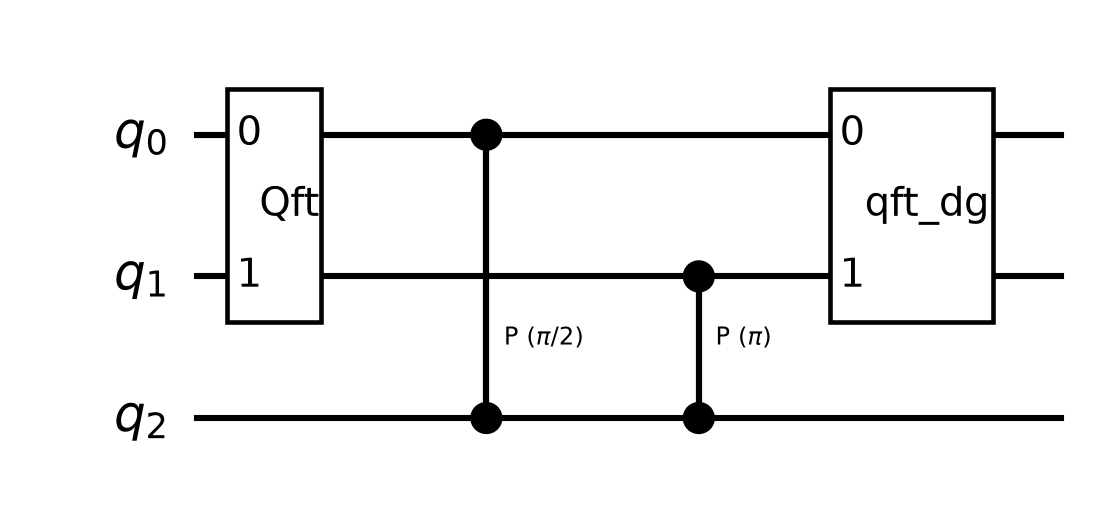
\includegraphics[width=\linewidth,height=3.6cm,keepaspectratio]{semisumador_qft.png}
\column{.42\textwidth}
\centering\textbf{Toffoli seguida de CNOT}\par\smallskip
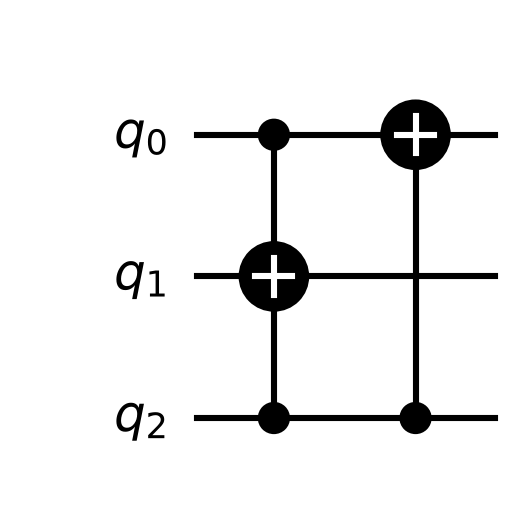
\includegraphics[width=\linewidth,height=3.6cm,keepaspectratio]{semisumador_toffoli.png}
\end{columns}
\smallskip
\idea{Se compara la transformación completa de los ocho estados de la base,
incluidos los que tienen el auxiliar inicial en uno.}
\fuente{Diagramas generados por Qiskit antes de la compilación.}
\end{frame}

% 15
\begin{frame}[shrink=0]{Cómo se obtienen las cinco funciones booleanas}
\setlength{\tabcolsep}{4pt}
\begin{columns}[T,onlytextwidth]
\column{.57\textwidth}
\small\renewcommand{\arraystretch}{1.35}
\begin{tabular}{@{}lll@{}}
\toprule
\textbf{Función} & \textbf{Antes del sumador} & \textbf{Después}\\\midrule
AND  & Identidad & Identidad\\
NAND & Identidad & $X$ en $q_1$\\
OR   & $X$ en $q_0$ y $q_2$ & $X$ en $q_1$\\
NOR  & $X$ en $q_0$ y $q_2$ & Identidad\\
XOR  & Identidad & SWAP $(q_0,q_1)$\\\bottomrule
\end{tabular}
\column{.39\textwidth}
\centering\small\renewcommand{\arraystretch}{1.4}
\begin{tabular}{@{}cc|ccccc@{}}
\toprule
$a$&$b$&\rotatebox{60}{AND}&\rotatebox{60}{NAND}&\rotatebox{60}{OR}&\rotatebox{60}{NOR}&\rotatebox{60}{XOR}\\\midrule
0&0&0&1&0&1&0\\
0&1&0&1&1&0&1\\
1&0&0&1&1&0&1\\
1&1&1&0&1&0&0\\\bottomrule
\end{tabular}
\end{columns}
\smallskip
\idea{Las mismas operaciones de preparación y salida se aplican a ambos diseños.
Las líneas restantes conservan información residual.}
\fuente{Función logic\_gate() en proyecto/experimento.py. OR y NOR se construyen con las leyes de De Morgan.}
\end{frame}

% 16
\begin{frame}[fragile]{El núcleo de la implementación en Qiskit}
\begin{columns}[T,onlytextwidth]
\column{.61\textwidth}
\begin{lstlisting}
from numpy import pi
from qiskit import QuantumCircuit
from qiskit.circuit.library import QFTGate

qc = QuantumCircuit(3)
qc.append(QFTGate(2), [0, 1])
qc.cp(pi / 2, 2, 0)
qc.cp(pi, 2, 1)
qc.append(QFTGate(2).inverse(), [0, 1])
\end{lstlisting}
\column{.35\textwidth}
\begin{block}{Interpretación}
\begin{enumerate}
\item QFT del acumulador.
\item Dos fases controladas por $b$.
\item QFT inversa para recuperar la suma.
\end{enumerate}
\end{block}
\small\texttt{half\_adder("Toffoli")} sustituye este núcleo por Toffoli y CNOT.
\end{columns}
\fuente{Versión comprobada: Qiskit \QiskitVersion{}. El código completo está en proyecto/experimento.py.}
\end{frame}

% 17
\begin{frame}[shrink=0]{Escalamiento: contador QFT frente a escalera AND}
\begin{columns}[T,onlytextwidth]
\column{.48\textwidth}
\begin{block}{Contador QFT: $N=2^k$ entradas}
\begin{itemize}
\item Reutiliza la primera entrada en el acumulador.
\item Añade $k$ auxiliares: \textbf{$N+k$ qubits}.
\item Obtiene $s=\sum_i x_i$ con $k+1$ bits.
\item Bit superior: AND. Bit inferior: paridad.
\end{itemize}
\end{block}
\column{.48\textwidth}
\begin{block}{Escalera de Toffoli}
\begin{itemize}
\item Calcula productos parciales de las entradas.
\item Usa $N-1$ auxiliares: \textbf{$2N-1$ qubits}.
\item Aplica $N-1$ Toffoli.
\item Conserva entradas y productos sin descomputarlos.
\end{itemize}
\end{block}
\end{columns}
\idea{Se compara AND; cada diseño deja distintos registros residuales.}
\fuente{Funciones population\_count() y and\_ladder(). Para N=8: 11 qubits QFT frente a 15 de la escalera.}
\end{frame}

% 18
\begin{frame}[shrink=0]{Validación de bits, fases y resultados}
\small

\begin{columns}[T,onlytextwidth]
\column{.50\textwidth}
\textbf{592 casos y 12 pruebas automatizadas}
\begin{itemize}
\item $5\times4\times2=40$ casos: cinco funciones, cuatro entradas y dos diseños.
\item $2(4+16+256)=\ValidationCases{}$ casos multientrada.
\end{itemize}
\centering\small
\begin{tabular}{@{}rlrr@{}}\toprule
$N$ & Diseño & Casos & $P_{\min}$\\\midrule
\ValidationRows\bottomrule
\end{tabular}
\column{.47\textwidth}
\textbf{Operadores completos de tres qubits}
\[
\varepsilon=\max_{ij}|(U_{\rm QFT}-U_{\rm Toffoli})_{ij}|.
\]
Unitariedad $U^\dagger U=I$ y comparación compilado/original: incluye fases de los ocho estados.
\smallskip\par
Tolerancia: $10^{-10}$. Error máximo: \texttt{\MaxUnitaryError{}}.
\smallskip\par
$P_{\min}$ de tablas: \MinTruthProbability{}.
QFT verifica peso de Hamming completo; Toffoli verifica AND.
\end{columns}
\fuente{Statevector y Operator; metricas.json, validacion.csv y tests. Probabilidades a seis decimales: diferencias numéricas de redondeo. Se valida el modelo ideal; la fidelidad QPU exige experimentos físicos.}
\end{frame}

% 19
\begin{frame}{Condiciones comunes de compilación}
\begin{columns}[T,onlytextwidth]
\column{.47\textwidth}
\begin{block}{Configuración}
\begin{itemize}
\item Python 3.12 y Qiskit \QiskitVersion{}.
\item Base de puertas: $\{U,\mathrm{CX}\}$.
\item Optimización: nivel 3.
\item Semilla: 42.
\item Conectividad completa.
\end{itemize}
\end{block}
\column{.49\textwidth}
\begin{block}{Qué se mide}
\begin{itemize}
\item Qubits, CX, profundidad y total de puertas.
\item Preparación y mediciones excluidas del costo.
\item Sin asumir entradas iniciales en cero:
\texttt{qubits\_initially\_zero=False}.
\end{itemize}
\end{block}
\end{columns}
\smallskip
\small\textbf{Permutaciones de salida:} un SWAP final puede representarse con
el etiquetado lógico. Se registra ese mapeo y se verifica con
\texttt{Operator.from\_circuit}.
\fuente{Configuración y permutaciones en metricas.json y CSV. Documentación oficial de Qiskit: compiler y Operator.}
\end{frame}

\section{Resultados propios}
% 20


% 21
\begin{frame}{Entradas en superposición: suma de dos bits uniformes}
\begin{columns}[c,onlytextwidth]
\column{.64\textwidth}
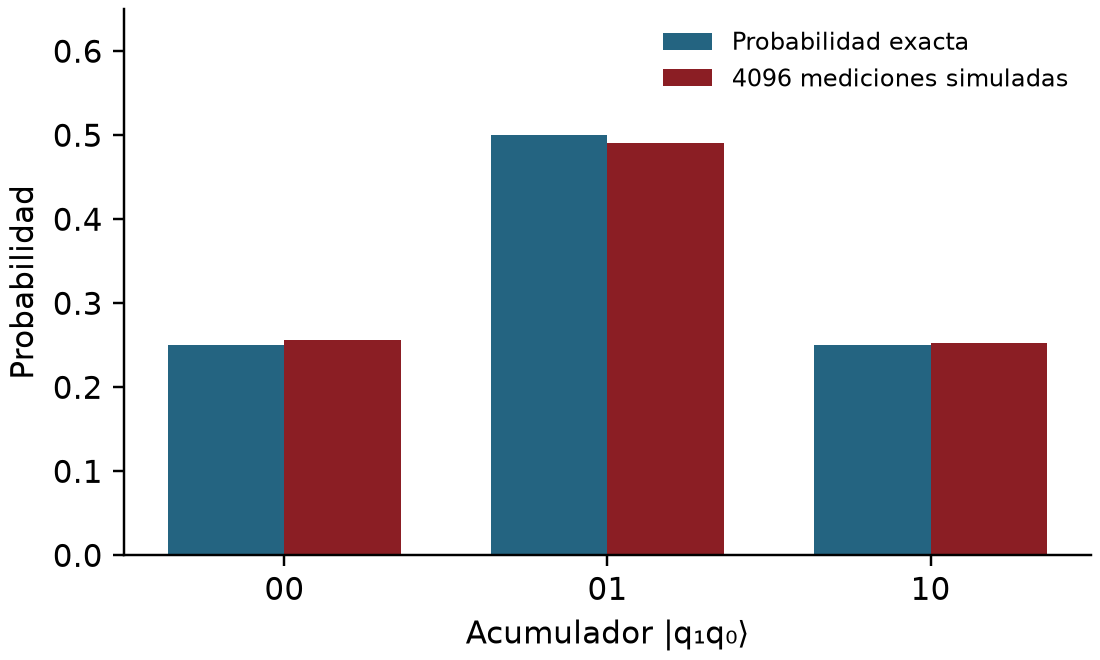
\includegraphics[width=\linewidth,height=5.5cm,keepaspectratio]{superposicion.png}
\column{.32\textwidth}
Se aplica $H$ a $q_0$ y $q_2$, seguido del semisumador QFT.
\smallskip
\begin{align*}
P(00)&=1/4,\\
P(01)&=1/2,\\
P(10)&=1/4.
\end{align*}
\small \textbf{4096 muestras}, semilla 42.\par
\smallskip Las diferencias se deben al muestreo finito.
\end{columns}
\fuente{Muestreo ideal en CPU con Statevector.sample\_counts. Se mide el acumulador q1q0.}
\end{frame}

% 22
\begin{frame}{Recursos AND: tablas y crecimiento con N}

\begin{columns}[c,onlytextwidth]
\column{.43\textwidth}
\centering\small
\begin{tabular}{@{}rlrrr@{}}\toprule
$N$ & Diseño & Qubits & CX & Prof.\\\midrule
\ScalingRows\bottomrule
\end{tabular}
\column{.55\textwidth}
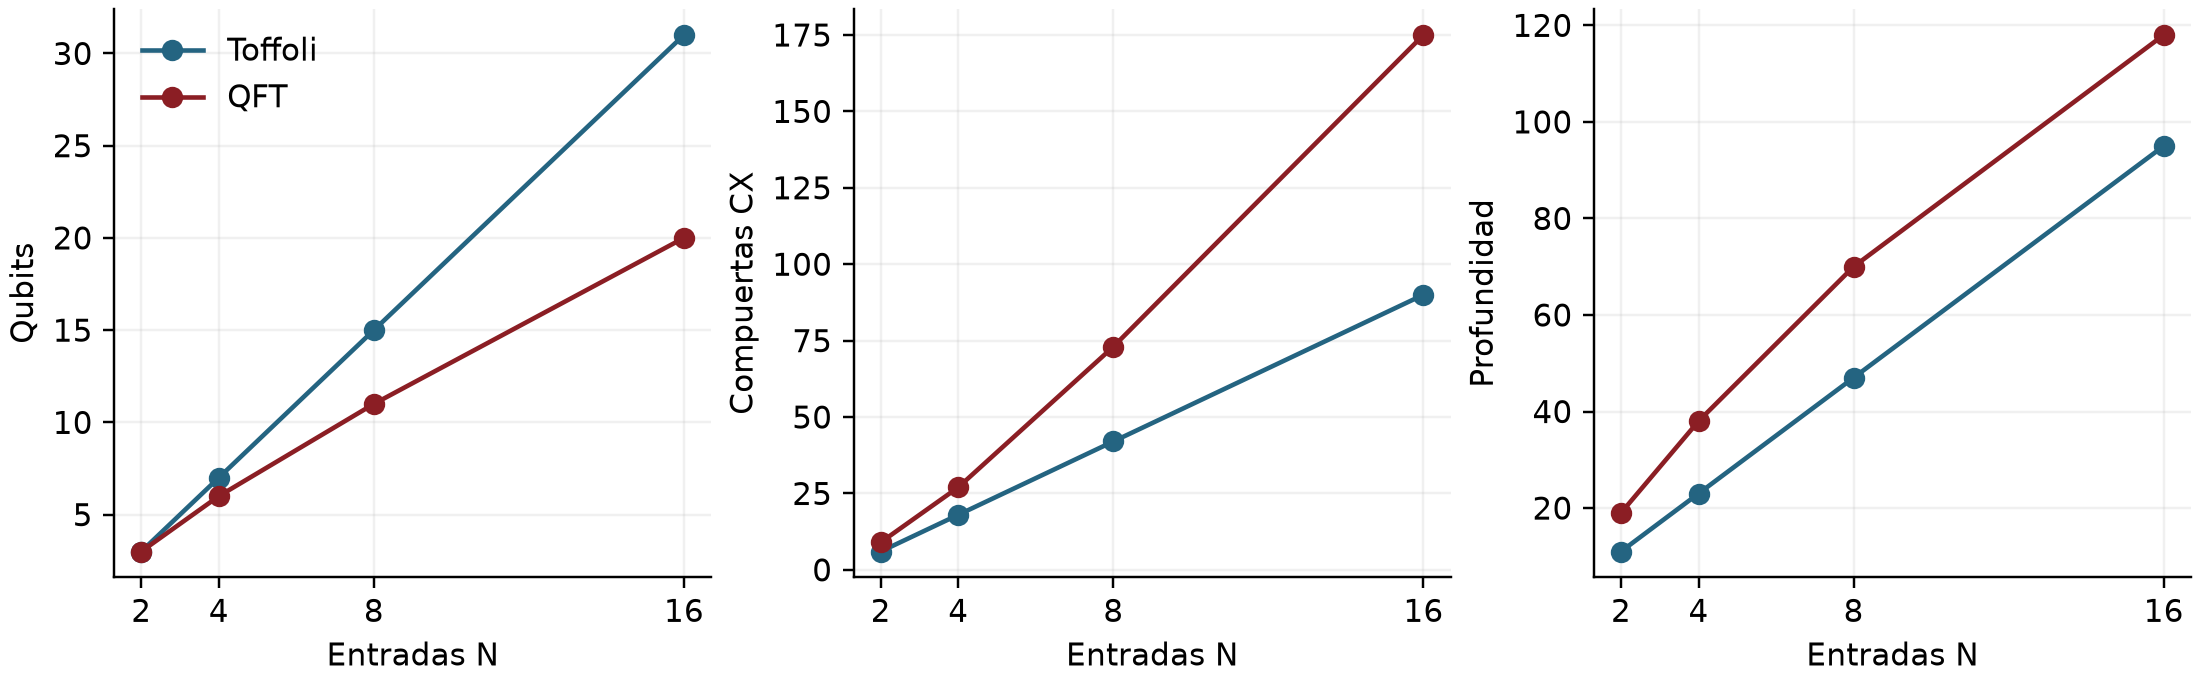
\includegraphics[width=\linewidth]{comparacion_recursos.png}
\textbf{$N=16$:} 20 frente a 31 qubits (11 menos: $35.5\%$); CX 175/90; profundidad 118/95.
\end{columns}
\smallskip
QFT reduce ancho para $N\geq4$ y devuelve además el conteo de población. La escalera usa menos CX y profundidad.
\fuente{escalamiento.csv; base y conectividad comunes. N=16 solo compilado, validación exhaustiva hasta N=8. Las curvas no representan tiempos ni fidelidades de hardware.}
\end{frame}

% 23


% 24
\begin{frame}{Limitaciones y siguiente etapa}
\begin{columns}[T,onlytextwidth]
\column{.48\textwidth}
\begin{alertblock}{Límites del avance}
\begin{itemize}
\item Simulación sin ruido ni errores de lectura.
\item Sin enrutamiento de una QPU concreta.
\item Registros residuales distintos en multientrada.
\item Conteo CX no equivale a conteo $T$.
\end{itemize}
\end{alertblock}
\column{.48\textwidth}
\begin{block}{Trabajo pendiente}
\begin{itemize}
\item Evaluar ruido y conectividad física.
\item Comparar MCX de pocos auxiliares.
\item Estudiar QFT aproximada.
\item Incluir descomputación y limpieza de registros.
\end{itemize}
\end{block}
\end{columns}
\smallskip\small
\textbf{Lectura correcta del resultado:} una probabilidad ideal cercana a uno
no establece una ventaja experimental en hardware.
\fuente{Las extensiones enumeradas permanecen pendientes; no se atribuyen resultados de esos experimentos al avance.}
\end{frame}

% 25
\begin{frame}[fragile]{Conclusiones y entrega reproducible}
\begin{enumerate}
\item La plantilla común permite construir y validar \textbf{cinco funciones reversibles}.
\item QFT y Toffoli implementan el \textbf{mismo operador de semisumador}, incluidas sus fases.
\item El ahorro de qubits debe evaluarse junto con \textbf{CX, profundidad y limpieza de registros}.
\end{enumerate}
\smallskip
\begin{block}{Cómo reproducir el avance desde la raíz del repositorio}
\begin{lstlisting}[language={},basicstyle=\ttfamily\footnotesize,frame=none]
.venv/bin/python -m pytest -q
.venv/bin/python -m proyecto.experimento
make informe presentacion
\end{lstlisting}
\end{block}
\small Código: \texttt{proyecto/experimento.py}. Datos y figuras:
\texttt{informe/latex/resultados/}.\par
\smallskip\textbf{Entrega: artículo, proyecto Qiskit, datos, pruebas y estas diapositivas.}
\end{frame}

\appendix
\section{Material de apoyo}
% 26
\begin{frame}[shrink=0]{Apoyo: recursos de las cinco funciones de dos entradas}
\begin{columns}[c,onlytextwidth]
\column{.51\textwidth}
\centering\footnotesize\renewcommand{\arraystretch}{1.05}
\begin{tabular}{@{}llrrr@{}}
\toprule
Función & Diseño & CX & Prof. & Total\\\midrule
\TwoInputRows
\bottomrule
\end{tabular}
\column{.45\textwidth}
\begin{block}{Cómo interpretar la tabla}
\begin{itemize}
\item Todos usan tres qubits.
\item Se compara la plantilla completa, con su información residual.
\item El compilador registra las permutaciones de salida.
\end{itemize}
\end{block}
\small Un XOR que solo actualiza un objetivo puede construirse con dos CNOT.
Esta plantilla no pretende ser una síntesis mínima para cada función.
\end{columns}
\fuente{Resultados propios de recursos\_dos\_entradas.csv. Total incluye puertas de uno y dos qubits de la base compilada.}
\end{frame}

% 27


% Las 16 referencias se leen de la misma base que el informe.
\begin{frame}[shrink=0]{Apoyo: cómo fundamentan el proyecto las fuentes añadidas}
\small
\begin{tabular}{@{}p{3cm}p{10.4cm}@{}}
\toprule
Fuente & Aplicación y límite en este avance\\\midrule
Bennett (1973) & Reversibilidad y descomputación; la limpieza de auxiliares queda pendiente.\\
Barenco et al. (1995) & Universalidad de puertas de un qubit y CX; justifica una base común.\\
Cuccaro et al. (2004) & Sumador con un auxiliar; el ahorro frente a nuestra escalera no se generaliza a todos los diseños Toffoli.\\
Maslov (2016) & Fases relativas bajo condiciones específicas; se conservan Toffoli exactas.\\
Shende et al. (2006) & Síntesis y costo CNOT; no se implementa su algoritmo.\\
Coppersmith (2002) & QFT aproximada (informe de 1994); aquí se usa QFT exacta.\\
\bottomrule
\end{tabular}
\fuente{Revisión dirigida: 12 fuentes académicas y cuatro referencias oficiales de API.}
\end{frame}

\begin{frame}[allowframebreaks]{Referencias bibliográficas (16 fuentes)}
\scriptsize
\setbeamertemplate{bibliography item}[text]
\nocite{kaltehei2026,escanez2026,clarino2025,hajjdiab2024}
\nocite{nielsen2010,draper2000,qftdocs,statedocs,compiledocs,operatordocs}
\nocite{bennett1973,barenco1995,cuccaro2004,maslov2016,shende2006,coppersmith2002}
\bibliographystyle{IEEEtran}
\bibliography{../informe/latex/referencias}
\end{frame}
\end{document}
